\documentclass[14pt,aspectratio=169]{beamer}

\usepackage{pgfpages}
\usepackage{fancyvrb}

\usepackage{tikz}
\usepackage{pgfplots}

\usepackage{minted}
\usemintedstyle{tango}

\usepackage{graphicx}

\usetheme{auriga}
\usecolortheme{auriga}

\setbeamercolor{background canvas}{bg=lightgray}

% define some colors for a consistent theme across slides

\definecolor{red}{RGB}{181, 23, 0}
\definecolor{blue}{RGB}{0, 118, 186}
\definecolor{gray}{RGB}{146, 146, 146}

\title{Web Development: \\ Using Frameworks \\ to Program JavaScript}

\author{{\bf Gregory M. Kapfhammer}}

\institute[shortinst]{{\bf Department of Computer Science, Allegheny College}}

\begin{document}

{
  \setbeamercolor{page number in head/foot}{fg=background canvas.bg}
  \begin{frame}
    \titlepage
  \end{frame}
}

% Slide
%
\begin{frame}{Technical Question}
  %
  \hspace*{.15in}
  %
  \begin{minipage}{5in}
    %
    \vspace*{.5in}
    %
    \begin{center}
      %
      {\large How can I use JavaScript frameworks for back-end and front-end
      web development?}
      %
    \end{center}
    %
  \end{minipage}
  %
  \vspace{1ex}
  %
  \begin{center}
    %
    \small Let's learn how to use JavaScript frameworks to created advanced web
    applications! Since this week's material assumes prior knowledge, make sure
    to review all previous content about HTML, CSS, and JavaScript! \\
    %
  \end{center}
  %
\end{frame}

% Slide
%
\begin{frame}{Pros and Cons of Software Frameworks}
  %
  \begin{itemize}
    %
    \item {\bf Software Framework}: a reusable library of code and documentation
      that a developer uses to simplify, improve, and facilitate the process of
      creating an application
      %
      \vspace*{-.15in}
      %
    \item What are the pros and cons of JavaScript frameworks?
      %
      \begin{itemize}
        %
        \item {\bf Pro}: reusing a component reduces development time
          %
        \item {\bf Con}: understanding a reusable component takes time
          %
        \item {\bf Pro}: an active community can answer questions
          %
        \item {\bf Con}: framework popularity changes rapidly
          %
      \end{itemize}
      %
      \vspace*{-.25in}
      %
    \item You may pick a JavaScript framework, start to use it, and then decide
      it is not a good fit! Developers face technical constraints, so how do you
      pick the ``best'' framework?
      %
  \end{itemize}
  %
\end{frame}

% Slide
%
\begin{frame}{The JavaScript Ecosystem is Exploding!}
  %
  \begin{figure}
    \centering
    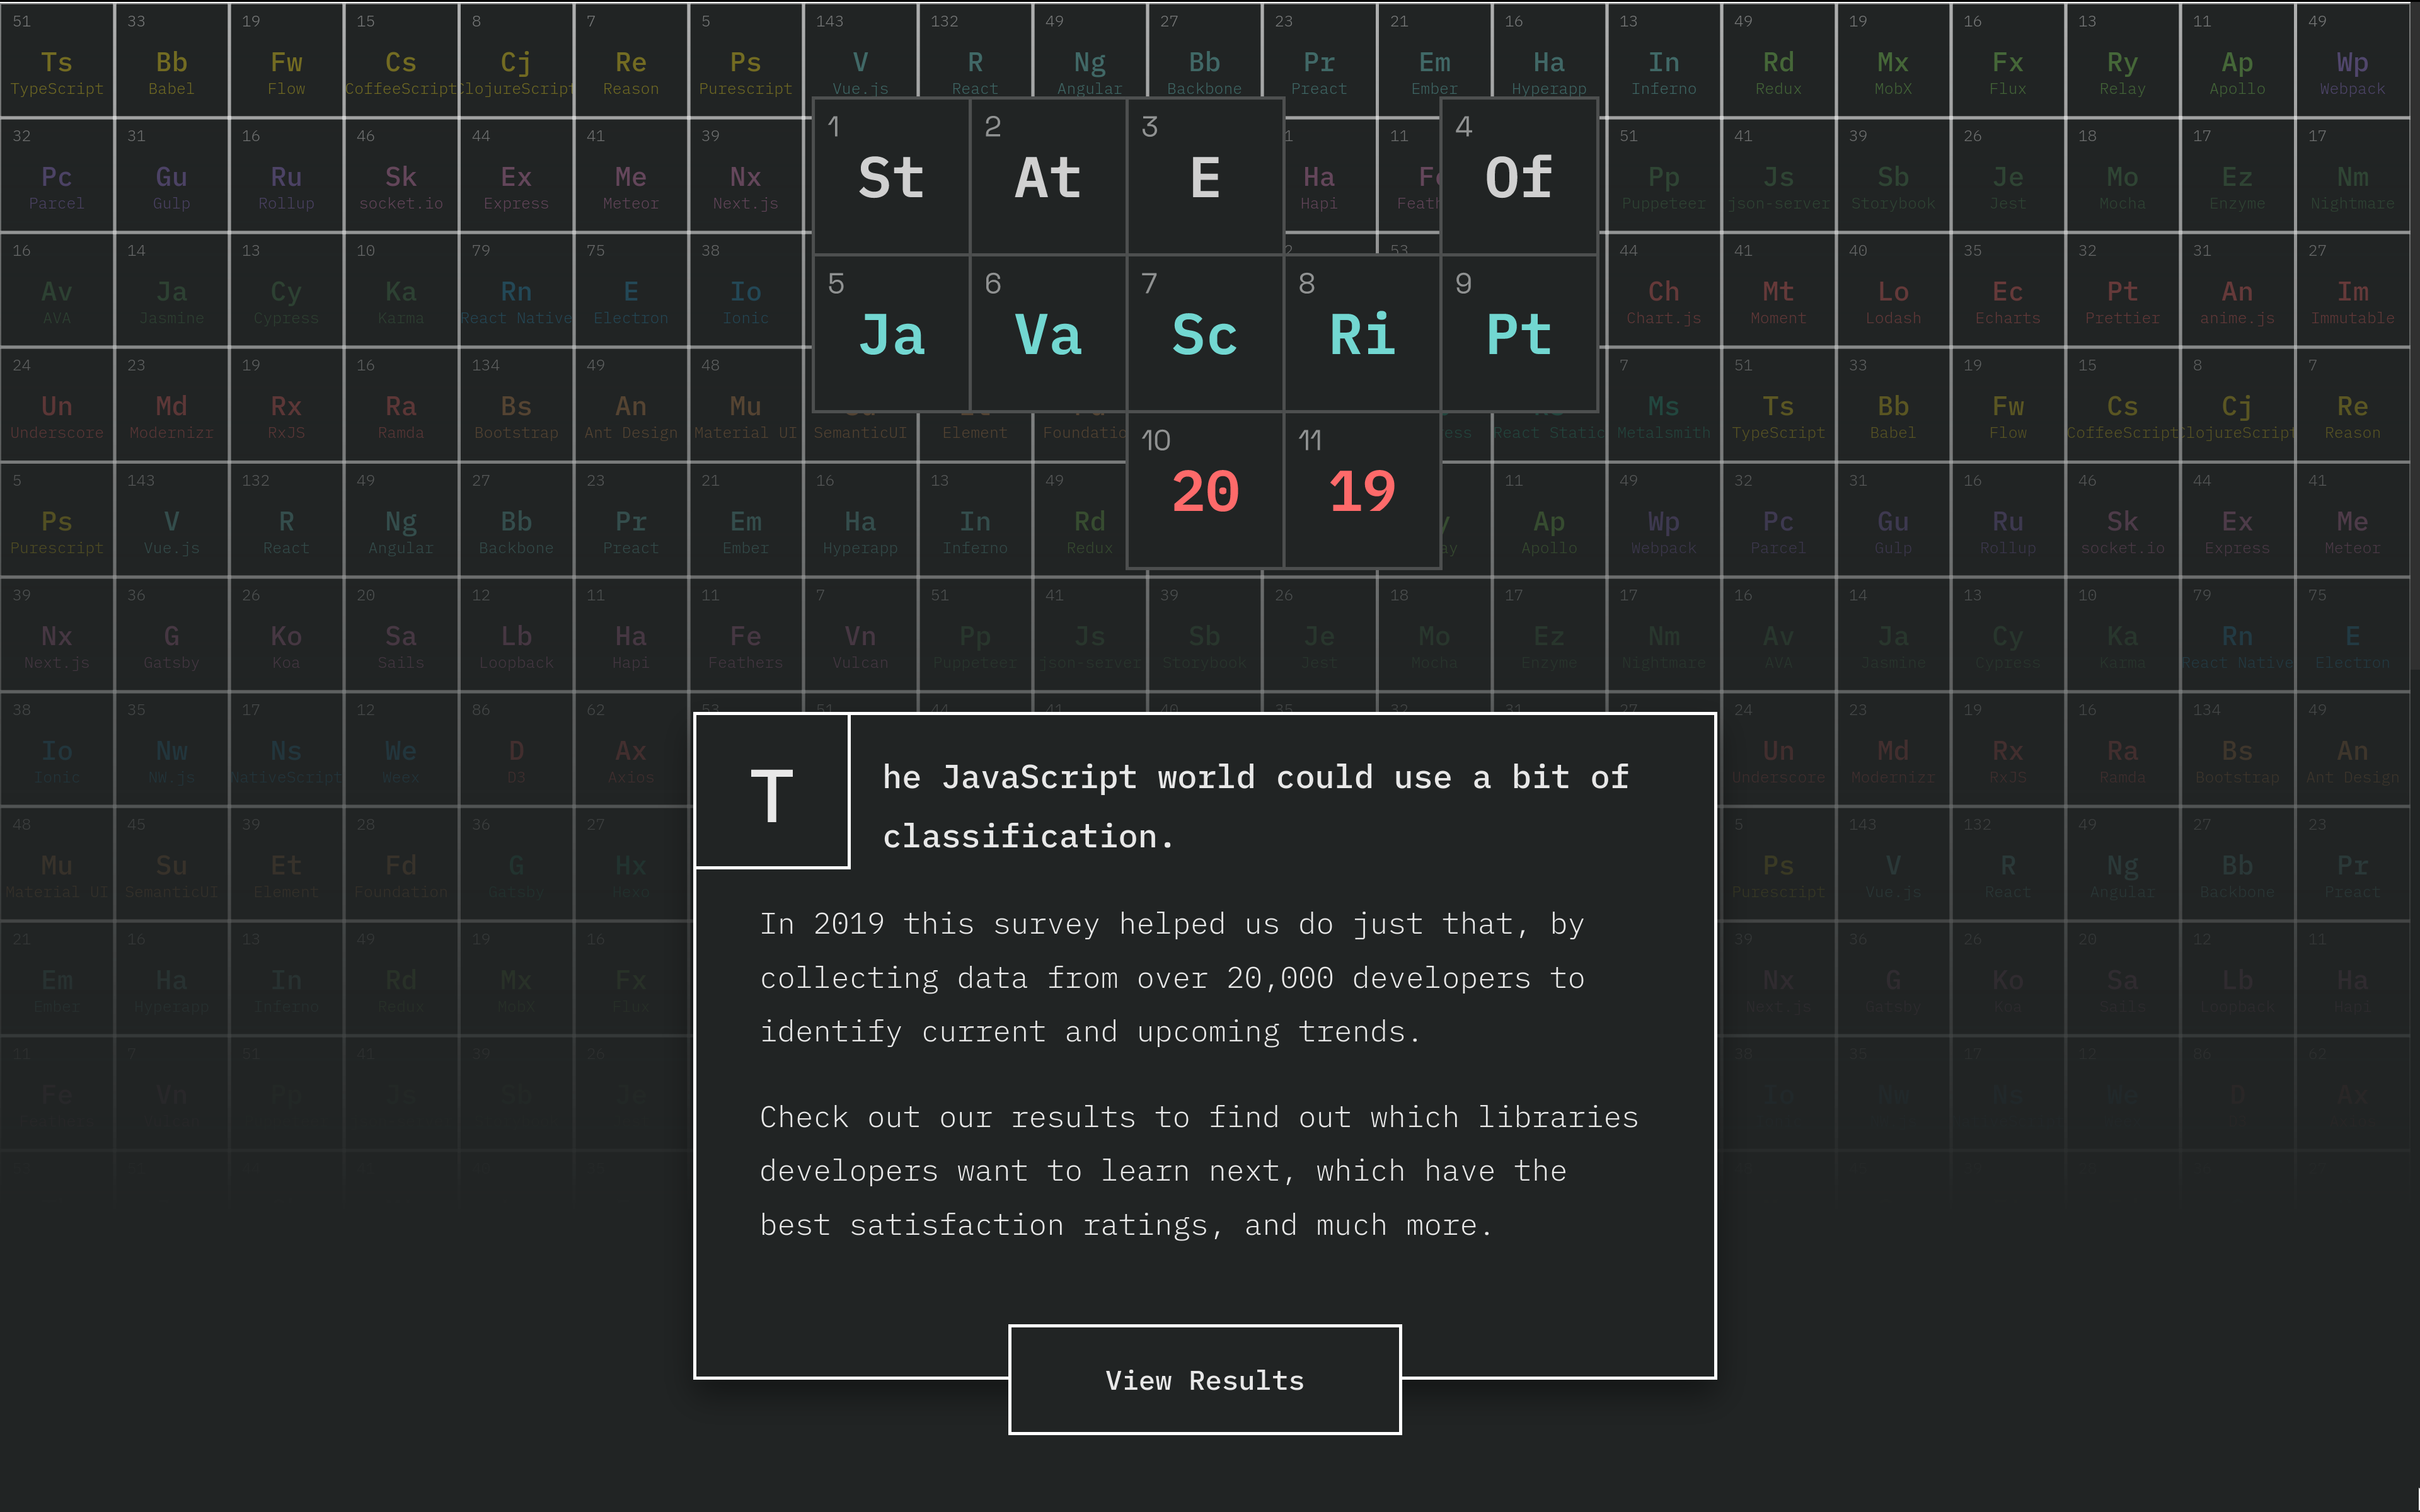
\includegraphics[scale=.080]{images/stateofjs.png}
    \caption{The figure's caption}
  \end{figure}
  %
\end{frame}

% Slide
%
\begin{frame}{Front-end JavaScript Frameworks}
  %
  \begin{itemize}
    %
    \item {\bf Ember}: an opinionated framework that uses a variant of the
      model-view-controller (MVC) design pattern to handle presentation, data
      binding, and routing in a web app
      %
      \vspace*{-.15in}
      %
    \item {\bf Angular}: another opinionated framework that also uses a variant
      of the model-view-controller (MVC) design pattern. Partially developed by
      Google, it leverages the TypeScript.
      %
      \vspace*{-.15in}
      %
    \item {\bf React}: a ``simpler'' framework that focuses on views instead of
      attempting to provide a full-featured MVC. Developed by Facebook, it
      uses an XML syntax called JSX.
      %
      \vspace*{-.15in}
      %
    \item What are the pros and cons of these frameworks?
      %
  \end{itemize}
  %
\end{frame}

% Slide
%
\begin{frame}{Back-end JavaScript Frameworks}
  %
  \begin{itemize}
    %
    \item {\bf MEAN Stack}: MongoDB, Express, Angular, Node.js
      %
      \vspace*{-.15in}
      %
    \item {\bf Node.js}: although it is complex, it shines in its support of
      high-performance push-based JavaScript applications
      %
      \vspace*{-.15in}
      %
    \item {\bf DIRT apps}: data-intensive real-time applications that require a
      high-performance asynchronous server
      %
      \vspace*{-.15in}
      %
    \item What are the pros and cons of using JavaScript for server-side
      programming in a web application?
      %
      \vspace*{-.15in}
      %
    \item Are there other programming languages that support server-side
      programming for the web? Yes, of course!
      %
  \end{itemize}
  %
\end{frame}

% Slide
%
\begin{frame}{npm: The Node Package Manager}
  %
  \begin{itemize}
    %
    \item How do you install a JavaScript package on your laptop?
      %
      \vspace*{-.15in}
      %
    \item The Node Package Manager is a command-line application that supports
      the installation of JavaScript packages
      %
      \vspace*{-.15in}
      %
    \item You will often use {\tt npm} even if you are not doing server-side
      JavaScript development!
      %
      \vspace*{-.15in}
      %
    \item For instance {\tt npm install --save quicklink} will install the
      Quicklink package on any web site!
      %
      \vspace*{-.15in}
      %
    \item How would you use the JavaScript package installed by {\tt npm}? How
      to ensure that JavaScript is available in HTML?
      %
  \end{itemize}
  %
\end{frame}

% Slide
%
\begin{frame}[fragile]
  \frametitle{Loading the Quicklink JavaScript Package}
  \normalsize
  \begin{minipage}{6in}
    \vspace*{.2in}
    \begin{minted}[mathescape, numbersep=5pt, fontsize=\large]{html}
<script src="dist/quicklink.umd.js">
</script>
<script>
quicklink.listen();
</script>
    \end{minted}
  \end{minipage}
  %
  \vspace*{.1in}
  %
  \begin{center}
    Make sure that the HTML points to the correct location \\
    Ensure that the {\tt dist} directory will be deployed on you site \\
    What if you do not want to arbitrarily start to listen? \\
  \end{center}
  %
\end{frame}

% Slide
%
\begin{frame}[fragile]
  \frametitle{Initializing the Quicklink JavaScript Package}
  \normalsize
  \begin{minipage}{6in}
    \vspace*{.2in}
    \begin{minted}[mathescape, numbersep=5pt, fontsize=\large]{html}
<script>
window.addEventListener('load', () => {
  quicklink.listen();
});
</script>
    \end{minted}
  \end{minipage}
  %
  \vspace*{.1in}
  %
  \begin{center}
    This embedded JavaScript is event-based programming \\
    Causes Quicklink to start listening on an event \\
    Quicklink will now start to pre-fetching suitable pages! \\
  \end{center}
  %
\end{frame}

% Slide
%
\begin{frame}{Summary of Pre-Fetching with Quicklink}
  %
  \begin{figure}
    \centering
    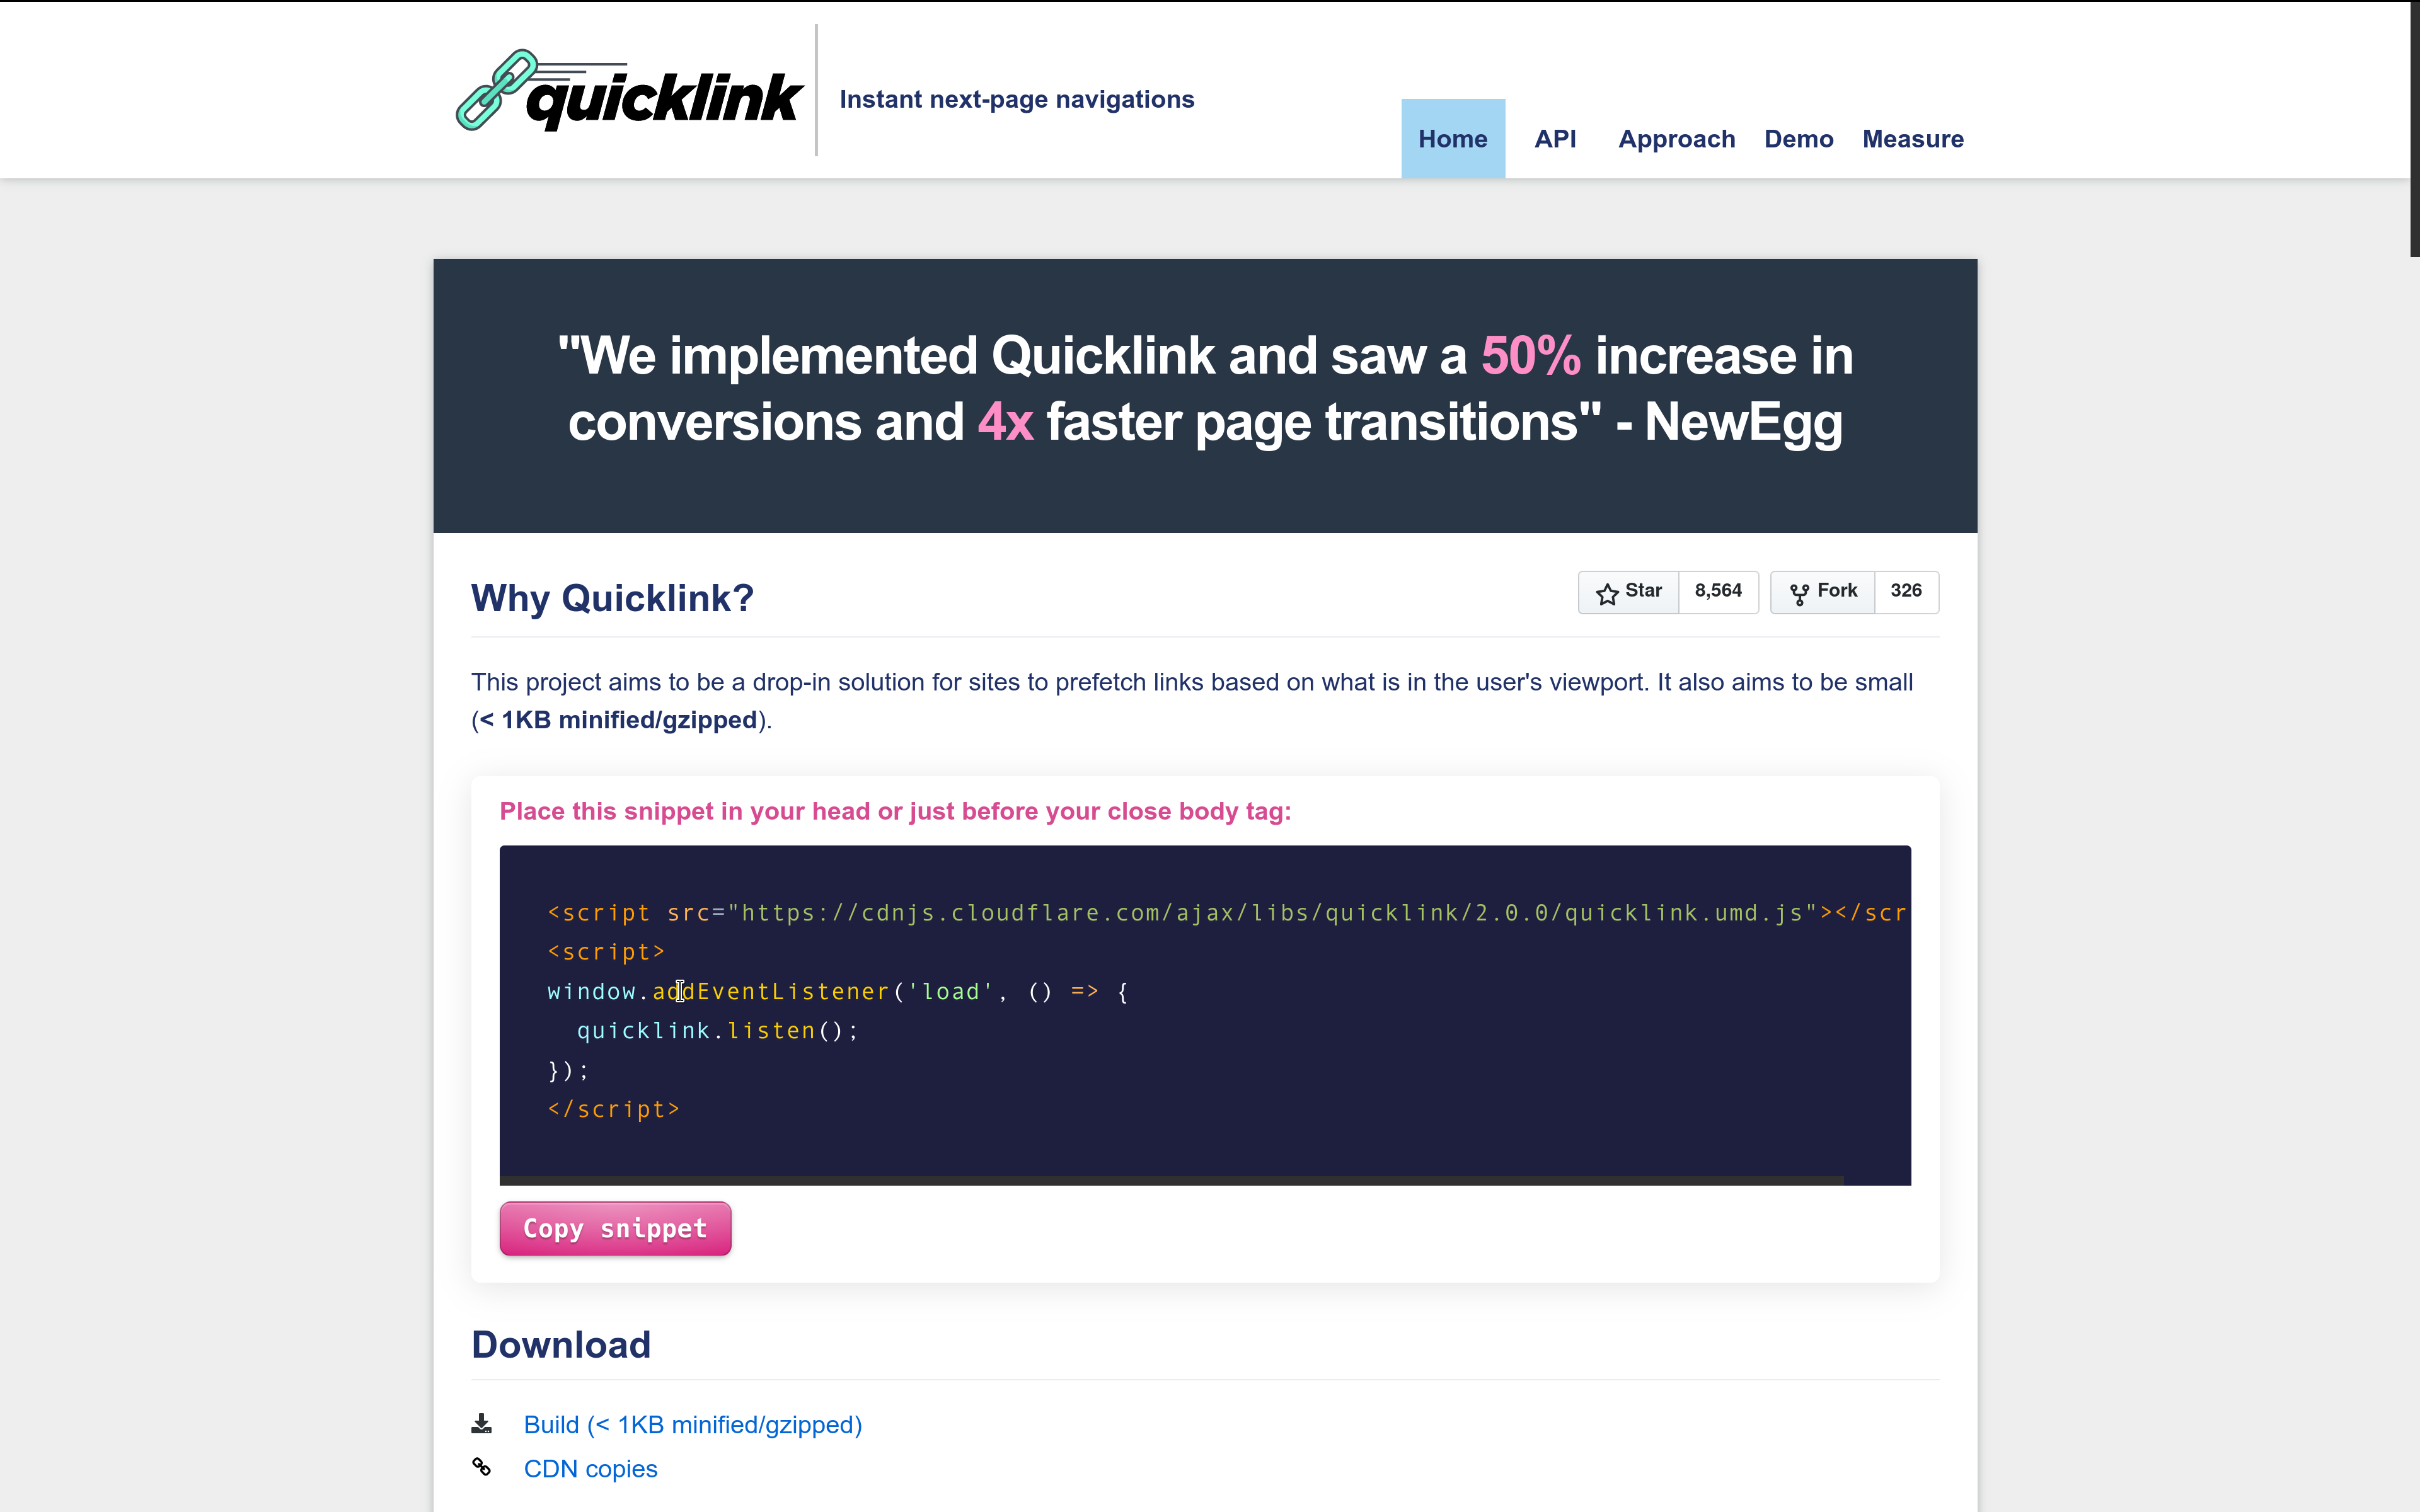
\includegraphics[scale=.08]{images/quicklink.png}
    \caption{The figure's caption}
  \end{figure}
  %
\end{frame}

% Slide
%
\begin{frame}{The React.js JavaScript Framework}
  %
  \begin{figure}
    \centering
    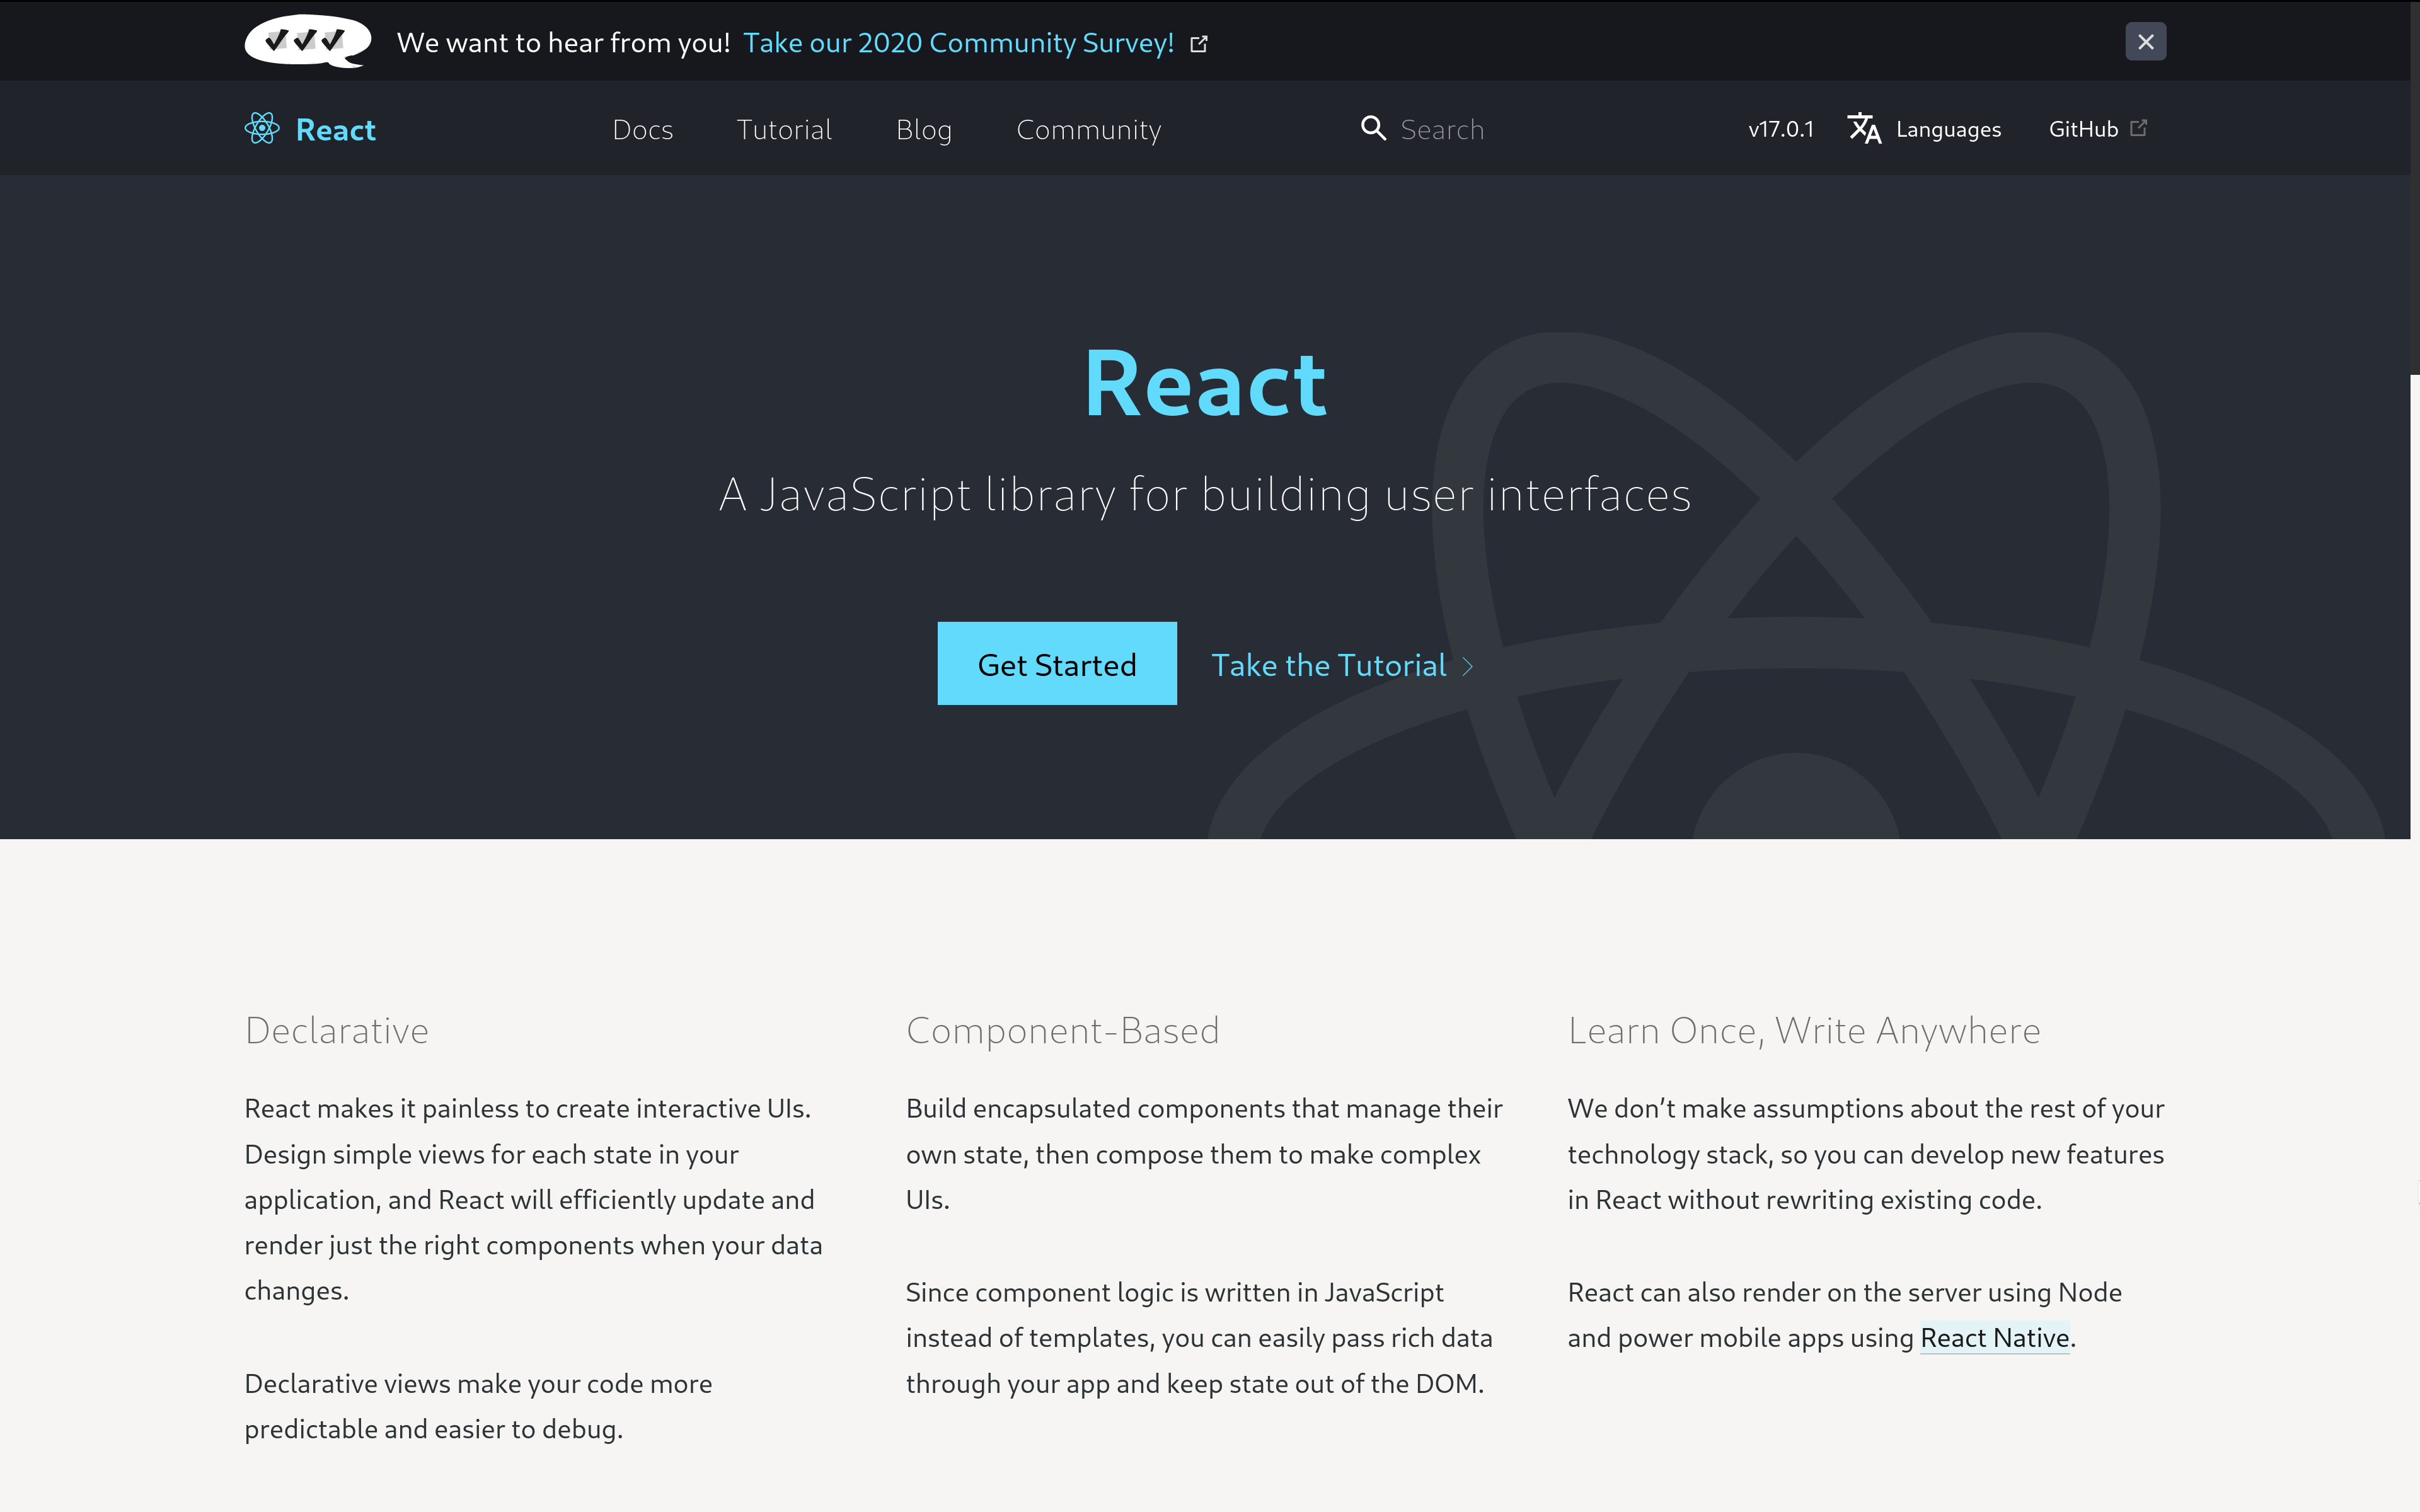
\includegraphics[scale=.08]{images/reactjs.png}
    \caption{The figure's caption}
  \end{figure}
  %
\end{frame}

% Slide
%
\begin{frame}{JavaScript-Based Presentations with Spectacle}
  %
  \begin{figure}
    \centering
    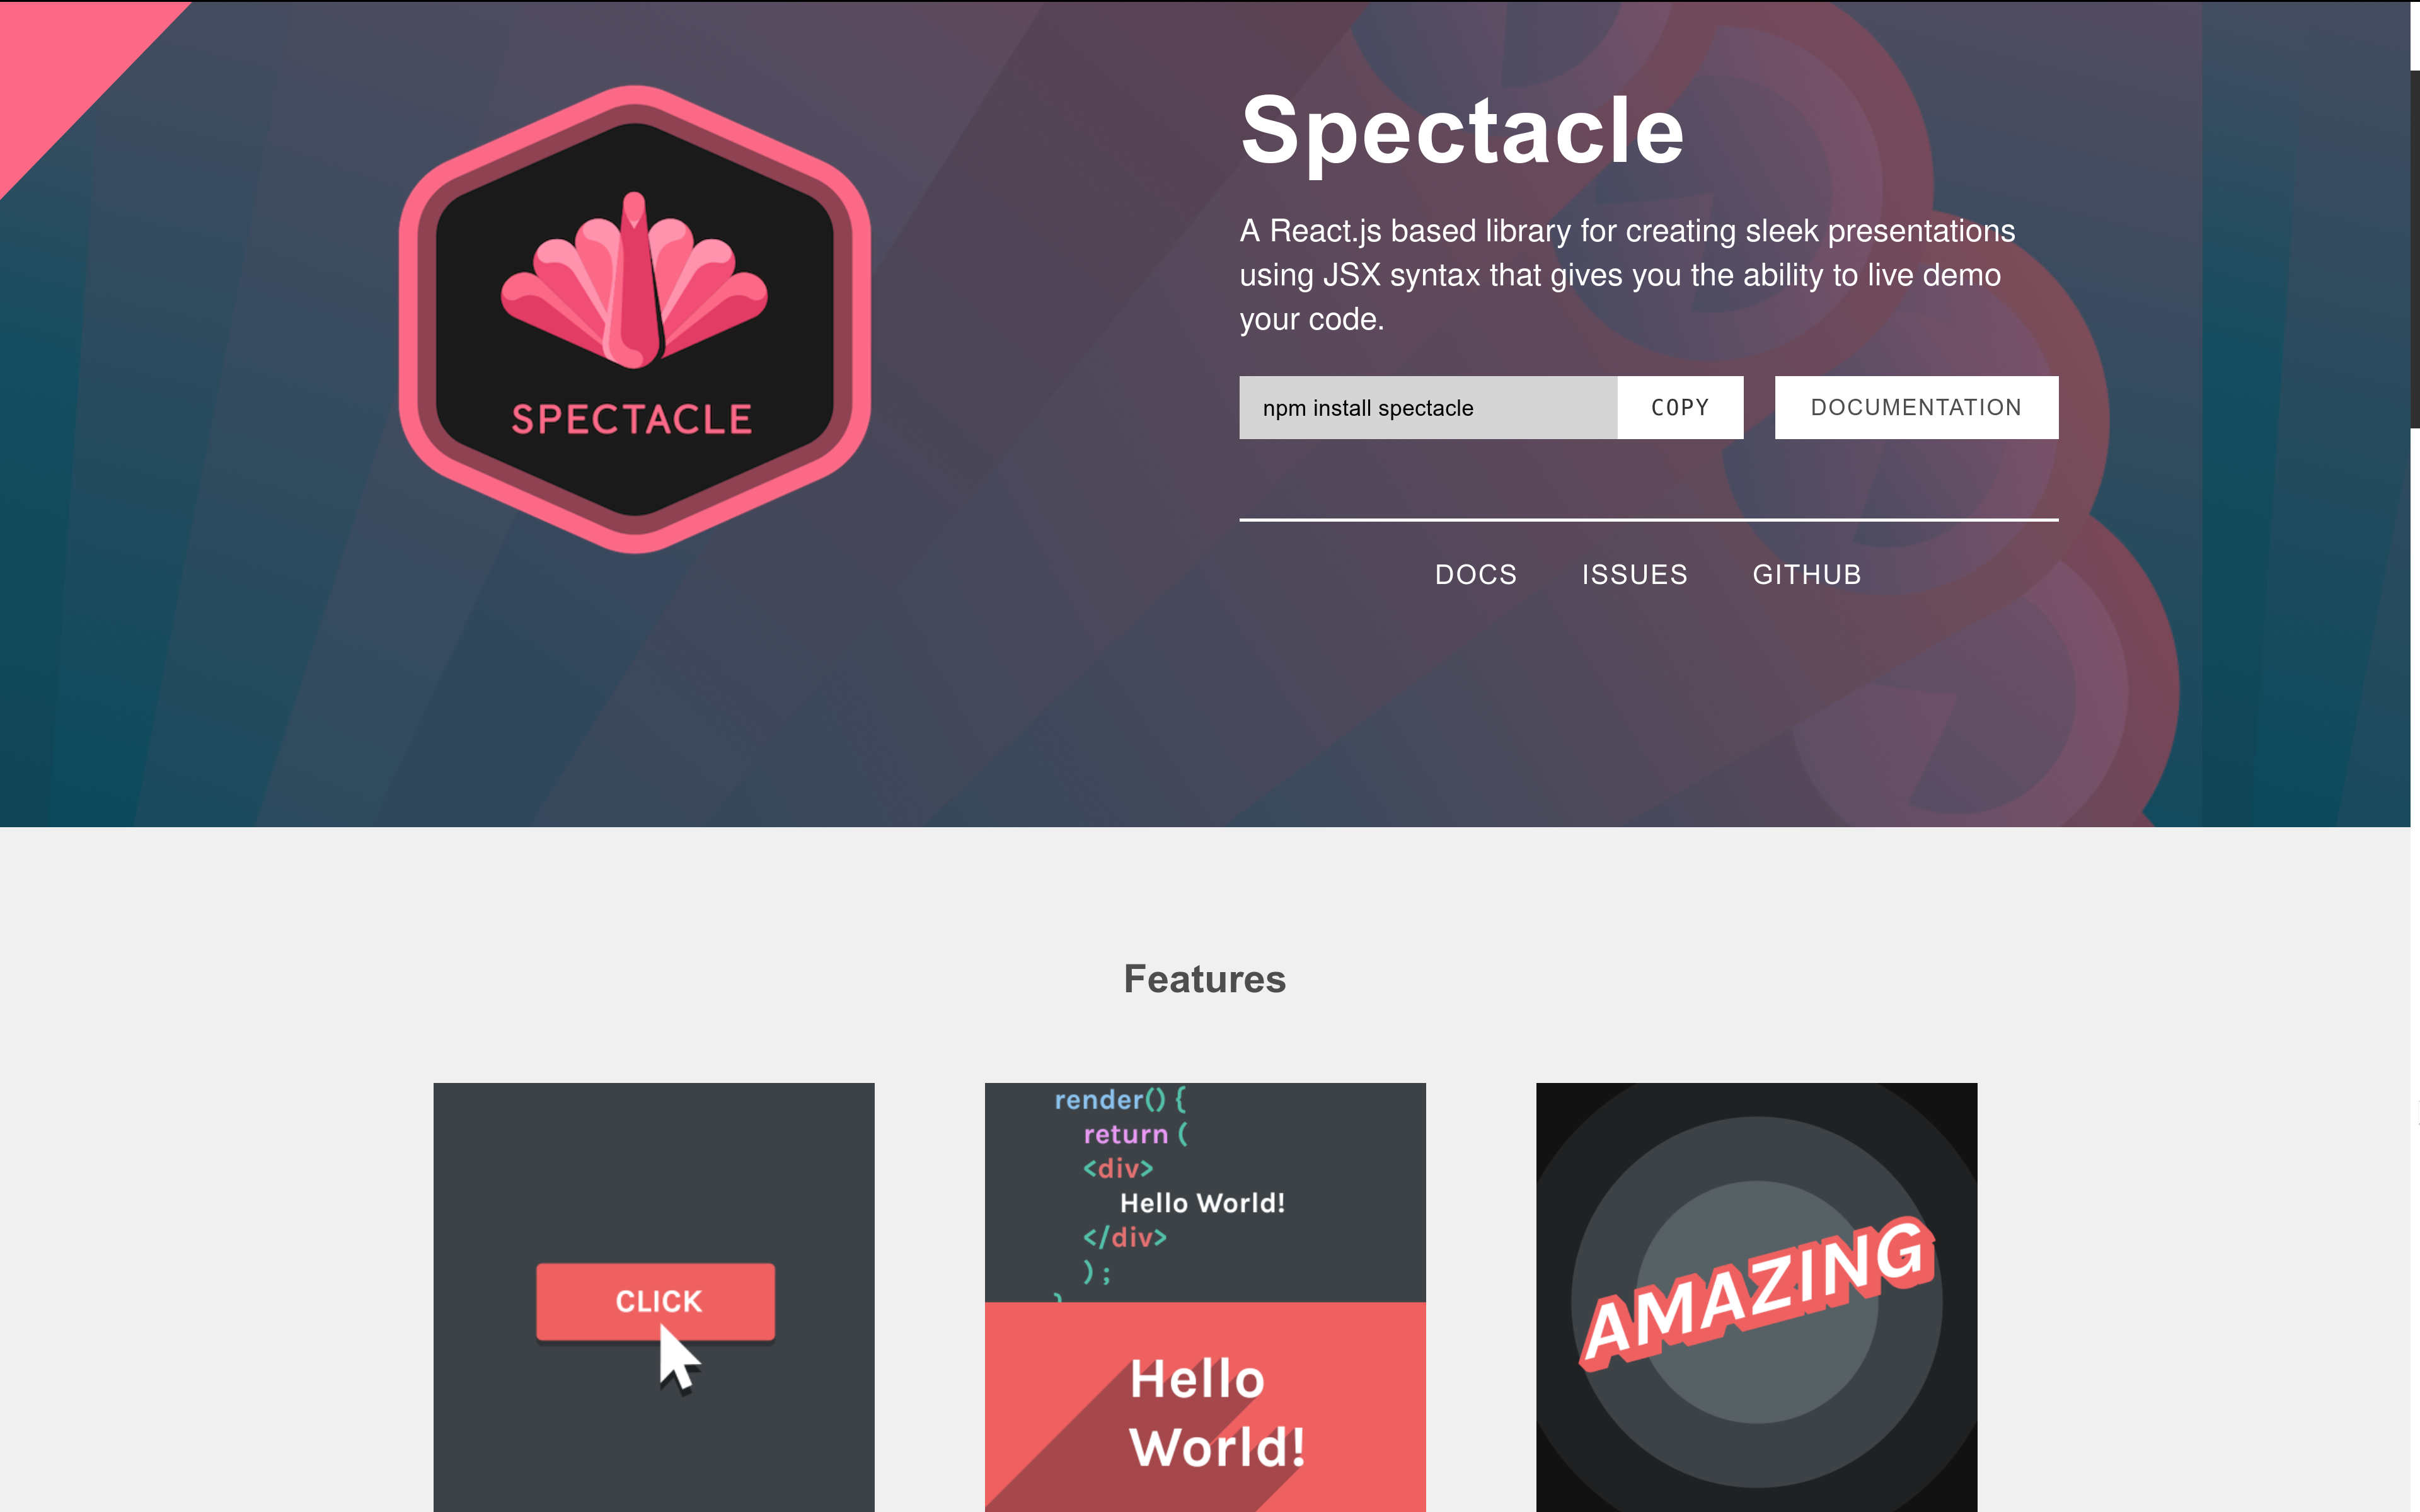
\includegraphics[scale=.08]{images/spectacle-javascript.png}
    \caption{The figure's caption}
  \end{figure}
  %
\end{frame}

% Slide
%
\begin{frame}[fragile]
  \frametitle{Importing React Components from Spectacle}
  \normalsize
  \hspace*{-.2in}
  \begin{minipage}{6in}
    \vspace*{.1in}
    \begin{minted}[mathescape, numbersep=5pt, fontsize=\large]{javascript}
import React, { Component } from 'react';
import styled from 'react-emotion';
import {
  Anim,
  Appear,
  BlockQuote,
  Cite,
  Code,
} from 'spectacle';
    \end{minted}
  \end{minipage}
  %
\end{frame}

% Slide
%
\begin{frame}[fragile]
  \frametitle{Importing React Components from Spectacle}
  \normalsize
  \hspace*{-.2in}
  \begin{minipage}{6in}
    \vspace*{.2in}
    \begin{minted}[mathescape, numbersep=5pt, fontsize=\large]{javascript}
const images = {
  TabCompletion: require('Complete.gif'),
  Linting: require('Linting.gif'),
  FixHardcode: require('FixHardcode.gif'),
  FuzzyFile: require('FuzzyFile.gif'),
};
preloader(images);
    \end{minted}
  \end{minipage}
  %
  \vspace*{.1in}
  %
  \begin{center}
    Pre-load images to be used later in the presentation \\
  \end{center}
  %
\end{frame}

% Slide
%
\begin{frame}[fragile]
  \frametitle{Declare Variables in a JavaScript Program}
  \normalsize
  \hspace*{.2in}
  \begin{minipage}{6in}
    \vspace*{.2in}
    \begin{minted}[mathescape, numbersep=5pt, fontsize=\large]{javascript}
var primary = '#FFF8DC';
var secondary = '#F4511E';
var secondarylight = '#FF6E40';
var tertiary = '#00897B';
var lighttext = '#9E9E9E';
var darktext = '#424242';
var lighttext = '#9E9E9E';
    \end{minted}
  \end{minipage}
  %
  \vspace*{.1in}
  %
  \begin{center}
    Global variables of colors for use throughout the program \\
  \end{center}
  %
\end{frame}

% Slide
%
\begin{frame}[fragile]
  \frametitle{Import a Package to Support Icon Reuse}
  \normalsize
  \hspace*{-.05in}
  \begin{minipage}{6in}
    \vspace*{.1in}
    \begin{minted}[mathescape, numbersep=5pt, fontsize=\normalsize]{javascript}
import { library } from
 '@fortawesome/fontawesome-svg-core'
import { FontAwesomeIcon } from
 '@fortawesome/react-fontawesome'
import { fab } from
 '@fortawesome/free-brands-svg-icons'
import { far } from
 '@fortawesome/free-regular-svg-icons'
import { fas } from
 '@fortawesome/free-solid-svg-icons'
    \end{minted}
  \end{minipage}
  %
  \vspace*{.05in}
  %
  \begin{center}
     Load existing packages for include FontAwesome icons
  \end{center}
  %
\end{frame}

% Slide
%
\begin{frame}[fragile]
  \frametitle{Creating a new Variable Containing HTML}
  \normalsize
  \hspace*{-.05in}
  \begin{minipage}{6in}
    \vspace*{.1in}
    \begin{minted}[mathescape, numbersep=5pt, fontsize=\normalsize]{javascript}
export const Twitter = () => (
    <FontAwesomeIcon icon={['fab', 'twitter']}
                     size="3x"
                     transform="left-2"
                     color='#00897B'/>
)
    \end{minted}
  \end{minipage}
  %
  \vspace*{.05in}
  %
  \begin{center}
     Colors the icons from the FontAwesome package for use in app \\
     Transforms the icons by changing their size and padding \\
     Creates a variable for use later in the React application! \\
     Questions about how to import and use React components?
  \end{center}
  %
\end{frame}

% Slide
%
\begin{frame}[fragile]
  \frametitle{Instantiating a React Component in JavaScript}
  \normalsize
  \hspace*{.2in}
  \begin{minipage}{6in}
    \vspace*{.2in}
    \begin{minted}[mathescape, numbersep=5pt, fontsize=\large]{javascript}
<Deck
  contentHeight={700}
  contentWidth={1024}
  transition={['slide']}
  transitionDuration={750}
  theme={theme}
  controls={false}
  progress={'none'}
>
    \end{minted}
  \end{minipage}
  %
\end{frame}

% Slide
%
\begin{frame}[fragile]
  \frametitle{Using React Components in JSX}
  \normalsize
  \hspace*{-.1in}
  \begin{minipage}{6in}
    \vspace*{.2in}
    \begin{minted}[mathescape, numbersep=5pt, fontsize=\large]{html}
<Layout>
  <Fill>
    <Text bold fit textColor="secondary">
      Gregory M. Kapfhammer
    </Text>
  </Fill>
</Layout>
    \end{minted}
  \end{minipage}
  %
  \vspace*{.1in}
  %
  \begin{center}
    These tags don't exist in HTML! These are React components! \\
  \end{center}
  %
\end{frame}

% Slide
%
\begin{frame}[fragile]
  \frametitle{Using React Components and Variables in JSX}
  \normalsize
  \hspace*{.1in}
  \begin{minipage}{6in}
    \vspace*{.2in}
    \begin{minted}[mathescape, numbersep=5pt, fontsize=\normalsize]{html}
<Layout>
  <Fit>
    <Twitter />
  </Fit>
  <Fit>
    <Text fill bold textSize="2em"
          textColor="tertiary">
      @GregKapfhammer
    </Text>
  </Fit>
</Layout>
    \end{minted}
  \end{minipage}
  %
\end{frame}

% Slide
%
\begin{frame}[fragile]
  \frametitle{Configuring React Components in JSX}
  \normalsize
  \hspace*{.1in}
  \begin{minipage}{6in}
    \vspace*{.1in}
    \begin{minted}[mathescape, numbersep=5pt, fontsize=\normalsize]{html}
<Layout>
  <Fill>
    <Backpack size={400}
              mood="blissful"
              color="#4DB6AC"/>
  </Fill>
  <Fill>
    <Cat size={400}
         mood="blissful"
         color="#FF8A65"/>
  </Fill>
</Layout>
    \end{minted}
  \end{minipage}
  %
\end{frame}

% Slide
%
\begin{frame}{Insights from Using React Components}
  %
  \begin{itemize}
    %
    \item React provides many valuable components for reuse
      %
      \vspace*{-.15in}
      %
    \item You normally must install each component using {\tt npm}
      %
      \vspace*{-.15in}
      %
    \item React uses a combination of JavaScript and XML called JSX
      %
      \vspace*{-.35in}
      %
    \item React feels like programming in both HTML and JavaScript!
      %
      \vspace*{-.35in}
      %
    \item Sometimes it is hard to know where to start! What components are
      available? Which ones should I pick? How do I create one? How do I use it?
      What if I have problems?
      %
      \vspace*{-.15in}
      %
    \item Questions about JavaScript programming with React?
      %
  \end{itemize}
  %
\end{frame}

\end{document}
